\documentclass{article}
\usepackage[francais]{babel}
\usepackage[utf8]{inputenc} % Required for including letters with accents
\usepackage[T1]{fontenc} % Use 8-bit encoding that has 256 glyphs
\usepackage{pythontex}
\usepackage{amsthm}
\usepackage{amsmath}
\usepackage{amssymb}
\usepackage{mathrsfs}
\usepackage{graphicx}
\usepackage{geometry}
\usepackage{stmaryrd}
\usepackage{tikz}
\usetikzlibrary{patterns}
%\usetikzlibrary{intersections}
\usepackage[cache=false]{minted}

\usepackage{stmaryrd}
%\usepackage{tikz}
%\usetikzlibrary{tikzmark}
\usepackage{empheq}
\usepackage{longtable}
\usepackage{booktabs} 
\usepackage{array}
\usepackage{pstricks}
\usepackage{pst-3dplot}
\usepackage{pst-tree}
\usepackage{pstricks-add}
\usepackage{upgreek}
%\usepackage{epstopdf}
\usepackage{eolgrab}
\usepackage{chngpage}
 \usepackage{calrsfs}
 % Appel du package pythontex 
\usepackage{pythontex}

\usepackage{algorithm2e}
\RestyleAlgo{algoruled}
  \SetKw{KwFrom}{from} 
\newenvironment{algo}{
\begin{algorithm}[H]
\DontPrintSemicolon \SetAlgoVlined}
{\end{algorithm}}



\usetikzlibrary{decorations.pathmorphing}
\def \de {{\rm d}}
\usepackage{color}
\usepackage{xcolor}
\newcommand{\mybox}[1]{\fbox{$\displaystyle#1$}}
\newcommand{\myredbox}[1]{\fcolorbox{red}{white}{$\displaystyle#1$}}
\newcommand{\mydoublebox}[1]{\fbox{\fbox{$\displaystyle#1$}}}
\newcommand{\myreddoublebox}[1]{\fcolorbox{red}{white}{\fcolorbox{red}{white}{$\displaystyle#1$}}}

\usepackage{xcolor}
%\setbeamercolor{background canvas}{bg=lightgray}
\usepackage{listings}
\definecolor{purple2}{RGB}{153,0,153} % there’s actually no standard purple
\definecolor{green2}{RGB}{0,153,0} % a

 \title{TP1 Analyse numérique (B1-TP1)}
\author{Ibrahim ALAME}
\date{28/02/2024}
\begin{document}
\maketitle

\section{Problème de tir}  
  On reprend ici le dernier exemple du cours (chapitre 2). On lance un projectile de masse $m$ avec une vitesse initiale $\vec{v_0}$ faisant un angle $\alpha$ avec l'axe horizontale. Le plan de tir est porté par un système d'axes $(O;x,y)$.
\begin{center}
 \begin{tikzpicture}[scale=0.5]
  \draw[->] (-0.1,0) -- (7.5,0)  node[right] {$\scriptstyle x$};
  \draw[->] (0,0.1) -- (0,-6) node[below] {$\scriptstyle y$};
   \draw[orange,dotted]  (0,-5.5) -- (7,-5.5) ;
   \draw[orange,dotted]  (7,0) -- (7,-5.5) ;
   \path[fill=black]  (1,-1.5) circle (1mm) [fill=gray];

   \draw [domain=0:5][line width=0.5] plot(\x,{-1-(\x-2)^2/2});

\end{tikzpicture}
 \end{center}

 L'équation différentielle du mouvement $\frac{\de^2 M}{\de t^2}=\vec g$ s'écrit  en coordonnées $x$, $y$ de M: 
  \[\left\{\begin{array}{l}
  x''=0\\
  y''=g
  \end{array}\right.\]
  On pose $z_0=x$, $z_1=y$, $z_2=x'$,$z_3=y'$. On a alors
  \[\left\{\begin{array}{l}
  z_0'=z_2\\
  z_1'=z_3\\
  z_2'=0\\
  z_3'=g
  \end{array}\right.\]
  On a donc un problème de Cauchy:
  \[\left\{\begin{array}{l}
  Z'=f(Z)\\
  Z_0 \mbox{ donné}
  \end{array}\right.\]
  où $Z=[z_0,z_1,z_2,z_3]$, $f(Z)=[z_2,z_3,0,g]$ et $Z_0=[x_0,y_0,v_0\cos(\alpha),v_0\sin(\alpha)]$
  
  Le schéma d'Euler s'écrit:
  
  \[\left\{\begin{array}{l}
  Z_{k+1}=Z_k+h\,f(Z_k)\\
  Z_0 =[10,200,50\cos(\pi/3),-50\sin(\pi/3)]
  \end{array}\right.\]
  où $h=0.1s$ et $g=9.81 m/s^2$.
  
  Le programme suivant applique la méthode d'Euler pour résoudre numériquement l'équation différentielle du problème et affiche le résultat en animation graphique dans une fenêtre {\tt tkinter} de hauteur $H=750$px et de largeur $W=750$px.
  
   Copiez et exécutez ce code:% dans votre compte {\tt repl.it}.
\begin{minted}[
mathescape,
framesep=2mm,
baselinestretch=1.2,
fontsize=\footnotesize,
linenos
]{python}
from tkinter import *
import numpy as np

# coordonnees initiales
x0, y0 = 10, 200
# vitesse initiale
alpha=np.pi/3
V0=50
# 'pas' du temps
h=0.1
z=np.array([x0,y0,V0*np.cos(alpha),-V0*np.sin(alpha)])
def f(z):
    return np.array([z[2],z[3],0,9.81])

def Euler():
    global z
    z=z+h*f(z)
    # deplacement de la balle a la nouvelle position
    can1.coords(balle, z[0], z[1], z[0] + 30, z[1] + 30)
    # La fenetre fen1 est actualisee en executant la
    # fonction Euler toutes les 10 millisecondes
    fen1.after(10, Euler)

# ========== Programme principal =============
# Creation de la fenetre principale :
fen1 = Tk()
fen1.title("Probleme de tir")
# creation du canvas :
H=W=750
can1 = Canvas(fen1, bg='dark grey', height=H, width=W)
can1.pack()
# creation de la balle
balle = can1.create_oval(x0, y0, x0 + 30, y0 + 30, width=2, fill='red')
# Lancement de la fonction Euler
Euler()
# demarrage de la boucle principale:
fen1.mainloop()

\end{minted} 
  
  Nous voulons que la balle rebondisse sur les bords de la fenêtre. Pour cela, à chaque fois que la boule touche un mur il faut inverser la vitesse normale. Par exemple: Si $z_1<0$ ou $z_1>H$ alors $z_3=-z_3$.

  Compléter le programme pour que la balle rebondisse aux 4 bords indéfiniment. 
  Faites tourner le programme pendant plus d'une minute. Que remarquez-vous?
  Modifiez le programme en passant à la méthode de Heun:
  \[\left\{\begin{array}{l}
  Z_{k+1}=Z_k+\frac h2\left[f(Z_k)+f(Z_k+h\,f(Z_k))\right]\\
  Z_0 
  \end{array}\right.\]
  Commentez le résultat obtenu.
  
  Dans cette question nous supposons que le projectile est soumis à une force de frottement proportionnelle à la vitesse, $\vec f=-k\vec v$. Écrire l'équation différentielle et le problème de Cauchy du mouvement. Actualiser le programme pour simuler la trajectoire réaliste de la balle en prenant $k=0.02$.
\section{Mouvement des planètes}  
\subsection{Soleil-Terre}
Nous savons que le mouvement d'un point matériel dans un champs à force centrale a lieu dans un plan. Le plan de mouvement est d'origine au coin gauche supérieur de l'écran conformément à la convention informatique. Le soleil occupe la position fixe $S(a,b)$. La terre est repérée par son centre $T(x,y)$ ses coordonnées sont solution de l'équation différentielle: $\frac{\de^2 T}{\de t^2}=\frac{GM_s}{r^2}\vec u$ où $r=ST$ et $\vec{u} =\frac{\overrightarrow{ST}}{ST}$, $G$ est la constante de gravitation $G=6.67\times 10^{-11} SI$ et$M_s$ est la masse du soleil $Ms=1.989\times 10^{30}$kg.
  \begin{center}
 \begin{tikzpicture}[scale=0.5]
  \draw[->] (-0.1,0) -- (7.5,0)  node[right] {$\scriptstyle x$};
  \draw[->] (0,0.1) -- (0,-6) node[below] {$\scriptstyle y$};
   \draw[orange,dotted]  (0,-5.5) -- (7,-5.5) ;
   \draw[orange,dotted]  (7,0) -- (7,-5.5) ;
   \path[fill=black]  (3,-3) circle (3mm) [fill=orange];
\path[fill=blue]  (5.5,-3) circle (2mm);
   \draw [domain=1.5:5.5][line width=0.5] plot(\x,{-3-sqrt(3*(1-(\x-3.5)^2/4) )});
   \draw [domain=1.5:5.5][line width=0.5] plot(\x,{-3+sqrt(3*(1-(\x-3.5)^2/4) )});

\end{tikzpicture}
 \end{center}

Comme pour le problème de tir, on pose $z_0=x$, $z_1=y$, $z_2=x'$,$z_3=y'$. On a alors
  \[\left\{\begin{array}{l}
  z_0'=z_2\\
  z_1'=z_3\\
  z_2'=-GM_s\frac{z_0-a}{\sqrt{(z_0-a)^2+(z_1-b)^2}^3}\\
  z_3'=-GM_s\frac{z_1-b}{\sqrt{(z_0-a)^2+(z_1-b)^2}^3}\\
  \end{array}\right.\]
   
Le programme suivant est une simulation du mouvement de la terre autour du soleil. Copiez, exécuter et commenter ce programme. Améliorer la résolution numérique en utilisant la méthode d'Euler amélioré puis la méthode de Range et Kutta.

\begin{minted}[
mathescape,
framesep=2mm,
baselinestretch=1.2,
fontsize=\footnotesize,
linenos
]{python}
from tkinter import *
import numpy as np

def f(z):
    r = np.sqrt((z[0] - a) ** 2 + (z[1] - b) ** 2)
    A = G * Ms / r ** 2
    Ax, Ay = -A * (z[0] - a) / r, -A * (z[1] - b) / r
    return np.array([z[2], z[3], Ax , Ay ])

def Euler():
    global z, h
    z=z+h*f(z)
    x1,y1 = z[0] // k, z[1] // k
    can1.coords(terre, x1, y1, x1 + 20, y1 + 20)
    fen1.after(1, Euler)

# ========== Programme principal =============
H, W = 4.0E11, 4.0E11
a, b = W / 2, H / 2  # centre de la terre
k = 4.0E8
# coordonnees initiales
x0, y0 = a + 1.47E11, H / 2
# vitesse initiale
V0 = 30200
alpha = np.pi / 2

Ms = 1.989E30
G = 6.67E-11

z = np.array([x0, y0, V0 * np.cos(alpha), -V0 * np.sin(alpha)])
# 'pas' du temps
h =  3600

fen1 = Tk()
fen1.title("Terre-Soleil")

can1 = Canvas(fen1, bg='dark grey', height=H // k, width=W // k)
can1.pack()

x1, y1 = z[0] // k, z[1] // k
terre = can1.create_oval(x1,y1 , x1 + 20, y1 + 20, width=2, fill='blue')
R = 6963400000
R=R*5
x1, y1=(a - R) // k, (b - R) // k
x2, y2=(a + R) // k, (b + R) // k
soleil = can1.create_oval(x1, y1, x2, y2, width=2, fill='yellow')

# Lancement de la fonction Euler
Euler()
# Boucle principale:
fen1.mainloop()
 \end{minted}
\subsection{Soleil-Terre-Lune}
 Les équations différentielles de la dynamique du système (S-T-L): soleil $S(a,b)$, terre $T(x_t,y_t)$  et lune $L(x_\ell,y_\ell)$, s'écrivent: 
 \[\left\{\begin{array}{l}
  \frac{\de^2 T}{\de t^2}=-\frac{GM_s}{r_1^2}\vec u_1-\frac{GM_l}{r_2^2}\vec u_2\\
  \frac{\de^2 L}{\de t^2}=-\frac{GM_s}{r_3^2}\vec u_3+\frac{GM_t}{r_2^2}\vec u_2
  \end{array}\right.\]
 
 On pose $z_0=x_t$, $z_1=y_t$, $z_2=x_t'$,$z_3=y'_t$, $z_4=x_\ell$, $z_5=y_\ell$, $z_6=x'_\ell$,$z_7=y'_\ell$. Préciser la fonction $f:\mathbb{R}^8\to\mathbb{R}^8$ de la formulation  de Cauchy: $Z'=f(Z)$ du système (S-T-L).
\begin{enumerate}
\item Écrire une nouvelle version du programme précédent permettant d'étudier le mouvement de la terre et de la lune autour du soleil.
\item Vérifier que l'année est $\simeq 365$ jours et que le mois est $\simeq 30$ jours.
\end{enumerate}

\begin{center}
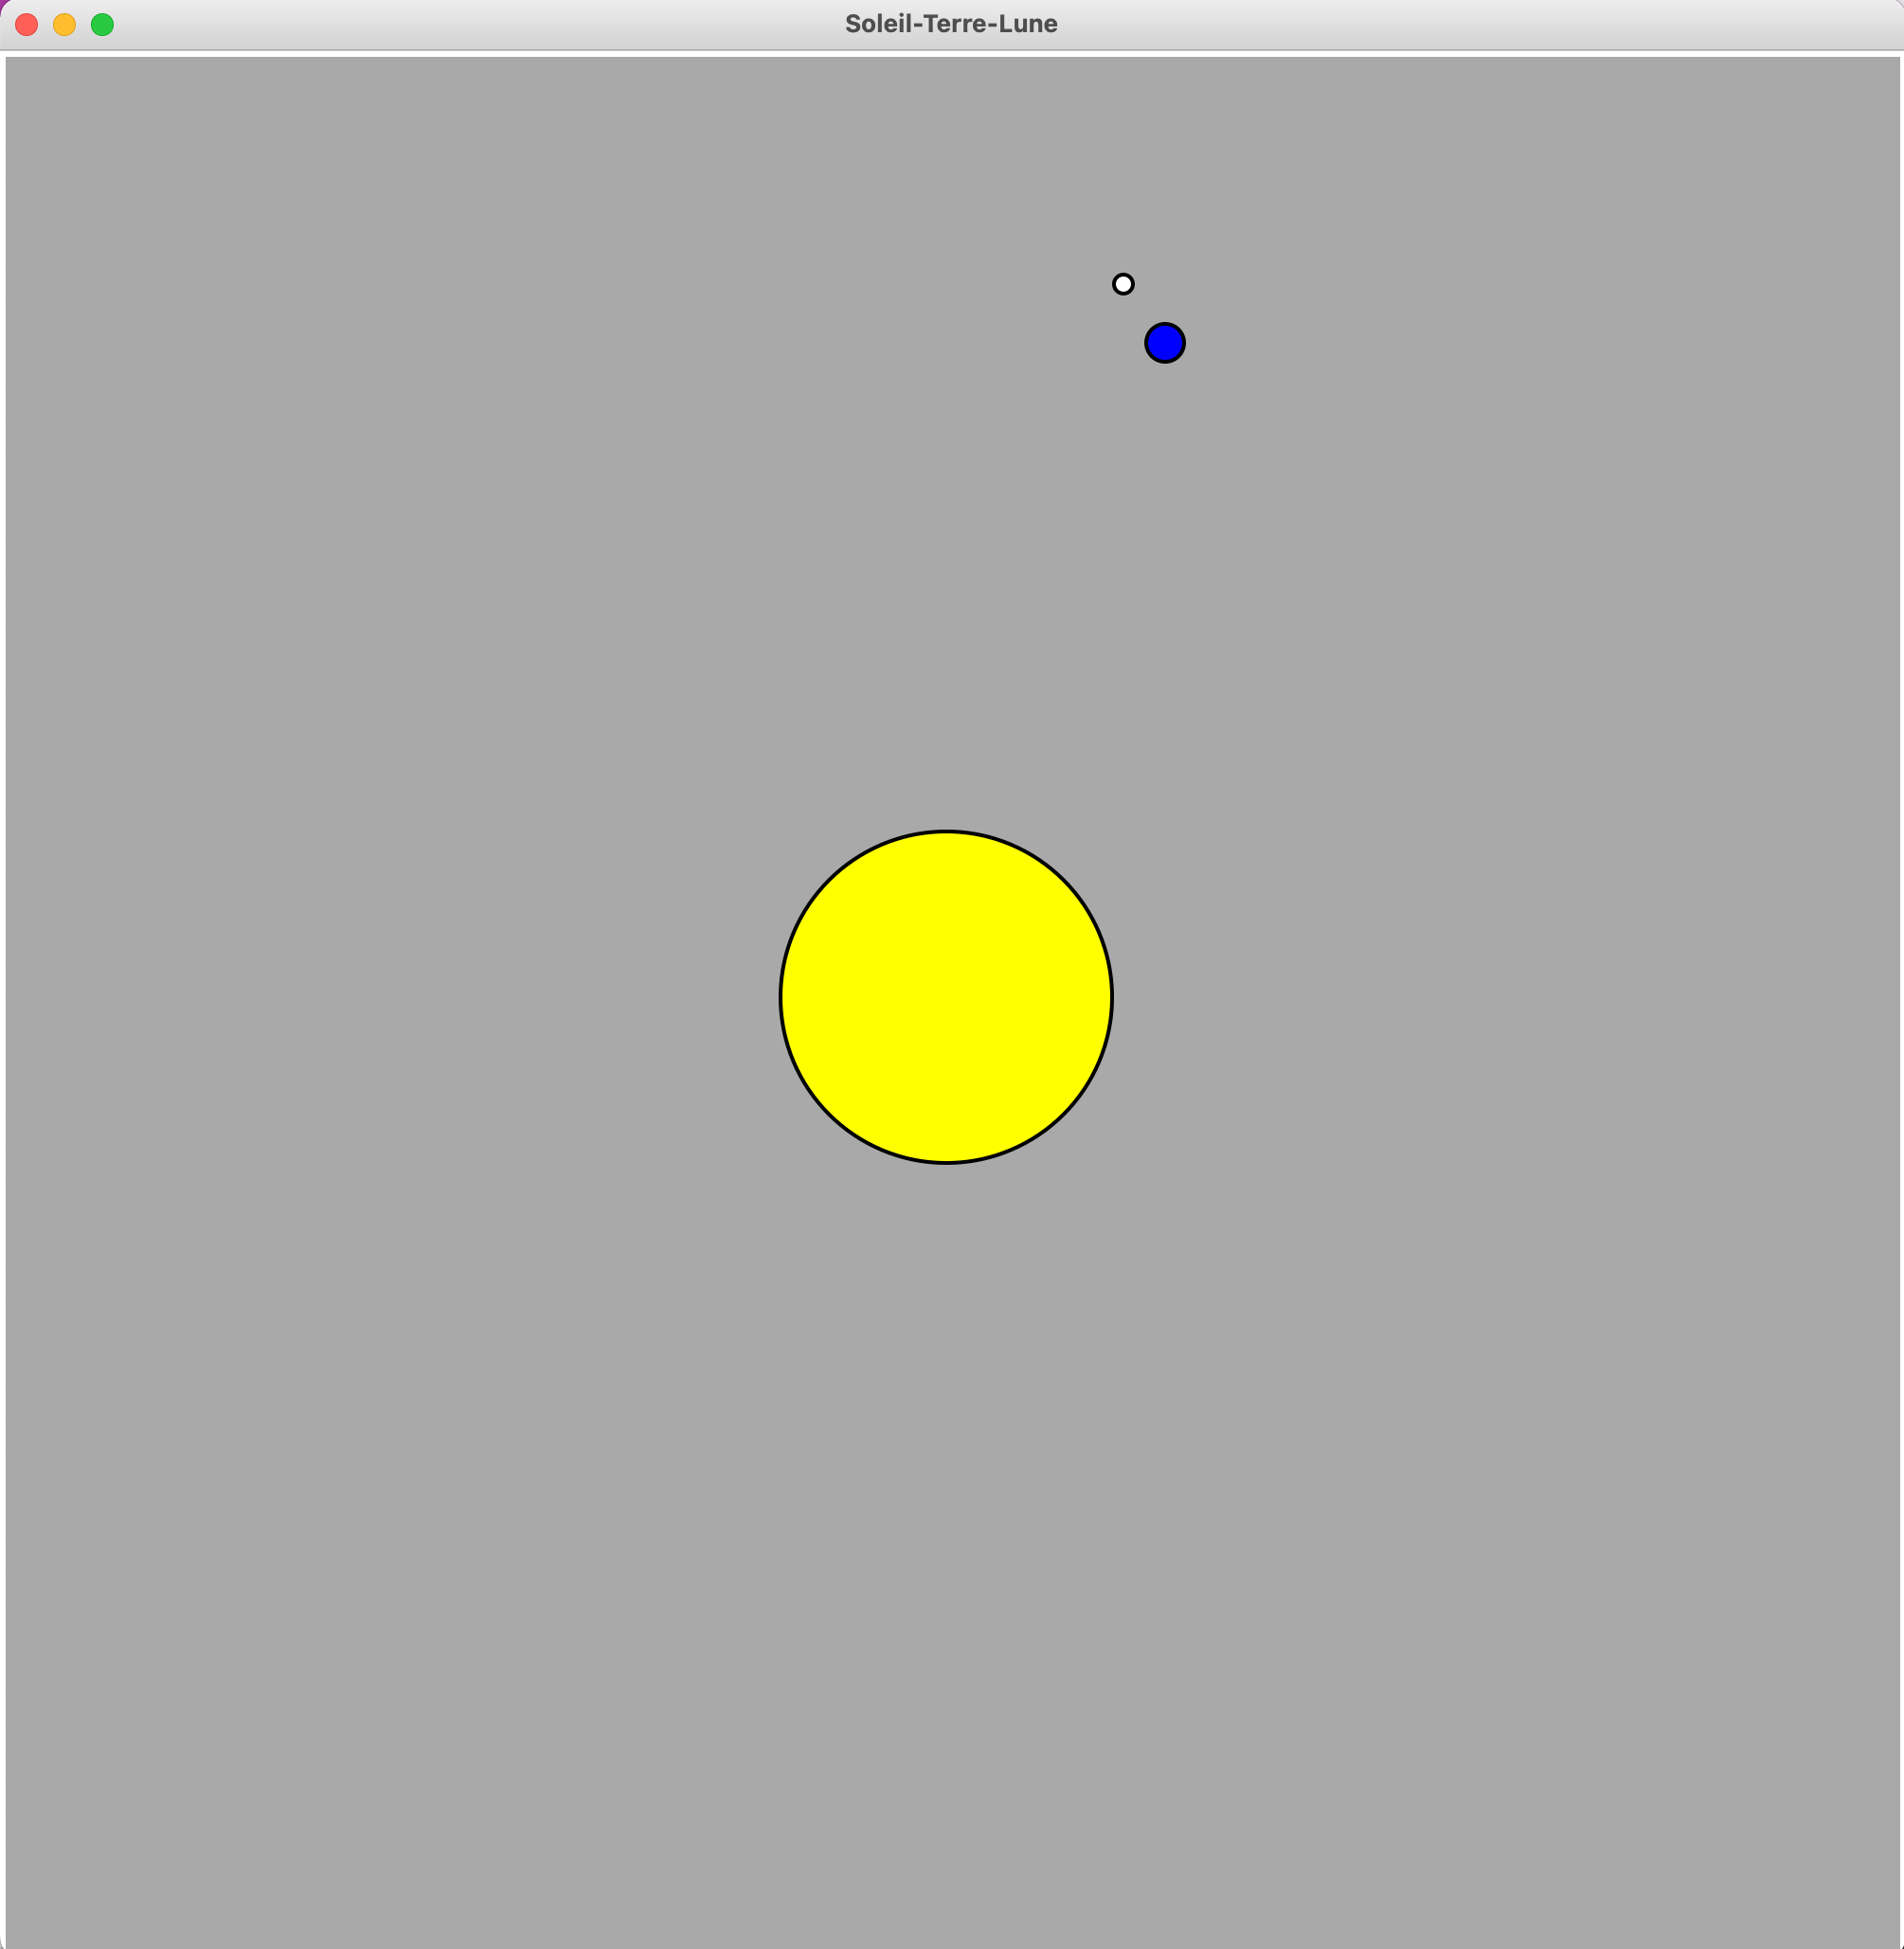
\includegraphics[width=10cm]{soleilTerreLune.png}
\end{center}

  \end{document}